\chapter{Experiments and Methods}\label{sec:experiments}
In the chapters \ref{sec:dummy_dataset} and \ref{sec:real_world_dataset} the synthetically generated dummy and real-world BSD datasets are presented. The generation of the datasets, the included domain shift and the resulting classification task are described. The proposed model architecture and the corresponding training are presented in the chapter \ref{sec:methods}.

\section{Dummy Dataset}\label{sec:dummy_dataset}
In the first step, different MMD-based domain adaptation approaches for PHM applications were evaluated on a synthetically generated dummy dataset. Such datasets are structured equally and show similar patterns as the corresponding real-world datasets. The complexity in such datasets and therefore, the difficulty of the corresponding tasks can be tuned arbitrarily. When analyzing new and unknown methods, dummy datasets help to visualize the data processing of the method. This gives deeper insight into the functionality of the method. Besides that, dummy datasets pre-evaluate the applicability of such methods for the corresponding real-world task.

In this thesis, a simple dummy dataset with a domain shift was created to investigate the ability of MMD-losses to facilitate the extraction of domain-invariant features in neural networks. Since one has to deal with irregularities, outliers and noise in real-world data, it is helpful to evaluate the MMD-loss on a dataset that is not disturbed by these effects. Similarly to PHM applications, the dummy dataset contained one-dimensional time sequences containing 1000 data points. In order to simulate a classification problem with two classes and two domains, the sequences were sampled from four cosine curves with characteristic amplitudes and frequencies. By adjusting the amplitude and frequency, the domain adaptation problem can be configured more or less difficult. The sampling process included certain randomness to allow variations between sequences of the same class and domain. For every sampled sequence, the characteristic amplitude and frequency were perturbed. This changed the underlying characteristic of each sequence. Besides that, noise was added to each of the 1000 data points. This is necessary to generate sequences similar to noisy real-world vibration signals. Exemplary samples for both classes and domains are shown in figure \ref{fig:samples_domain_class_dummy}.

\begin{figure}[H]
  \centering
  \includegraphics[width=.47\textwidth]{samples_domain_class_dummy/Source_Domain_Class_0_obs_0.pdf}
  \hspace{.3cm}
  \includegraphics[width=.47\textwidth]{samples_domain_class_dummy/Source_Domain_Class_1_obs_0.pdf}

  \vspace{.3cm}

  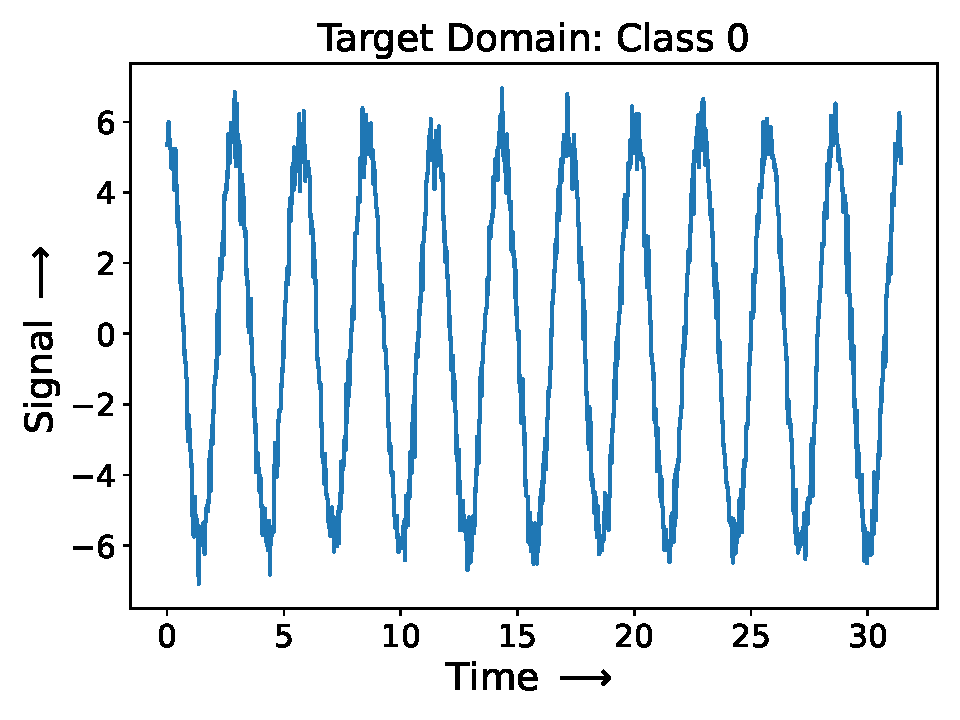
\includegraphics[width=.47\textwidth]{samples_domain_class_dummy/Target_Domain_Class_0_obs_0.pdf}
  \hspace{.3cm}
  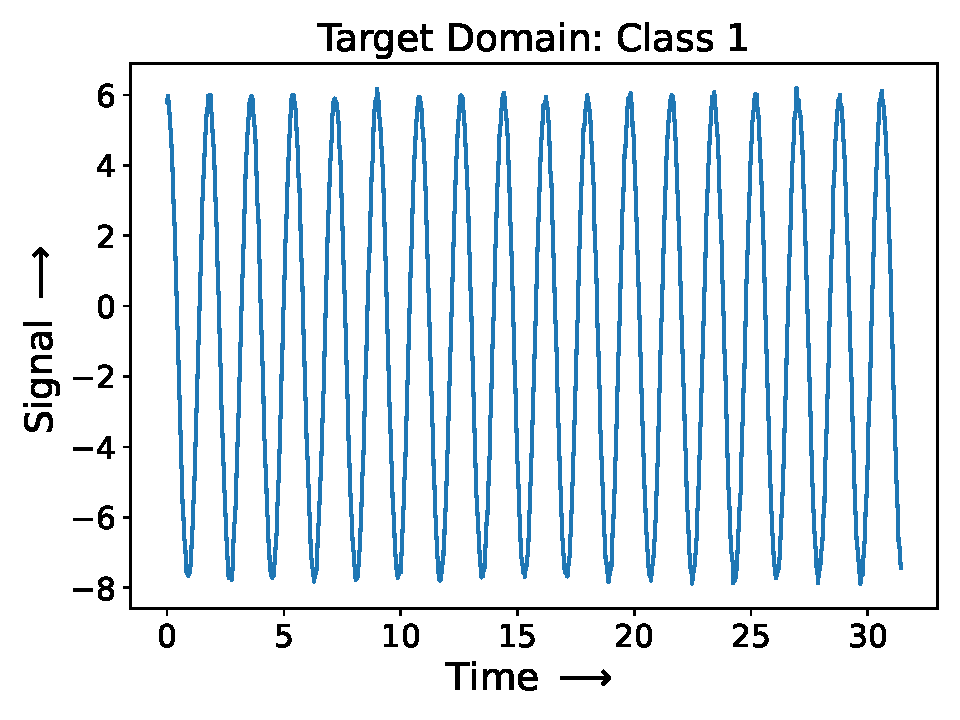
\includegraphics[width=.47\textwidth]{samples_domain_class_dummy/Target_Domain_Class_1_obs_0.pdf}

  \caption{Dummy data samples for all classes and domains}
  \label{fig:samples_domain_class_dummy}
\end{figure}

Figure \ref{fig:samples_domain_class_dummy_influence_noise} visualizes how the perturbation of the frequencies and amplitudes and the noise added to each data point, generate differences between samples of the same class and domain.

\begin{figure}[H]
  \centering
  \includegraphics[width=.47\textwidth]{samples_domain_class_dummy_influence_noise/Source_Domain_Class_0_obs_0.pdf}
  \hspace{.3cm}
  \includegraphics[width=.47\textwidth]{samples_domain_class_dummy_influence_noise/Source_Domain_Class_1_obs_0.pdf}

  \vspace{.3cm}

  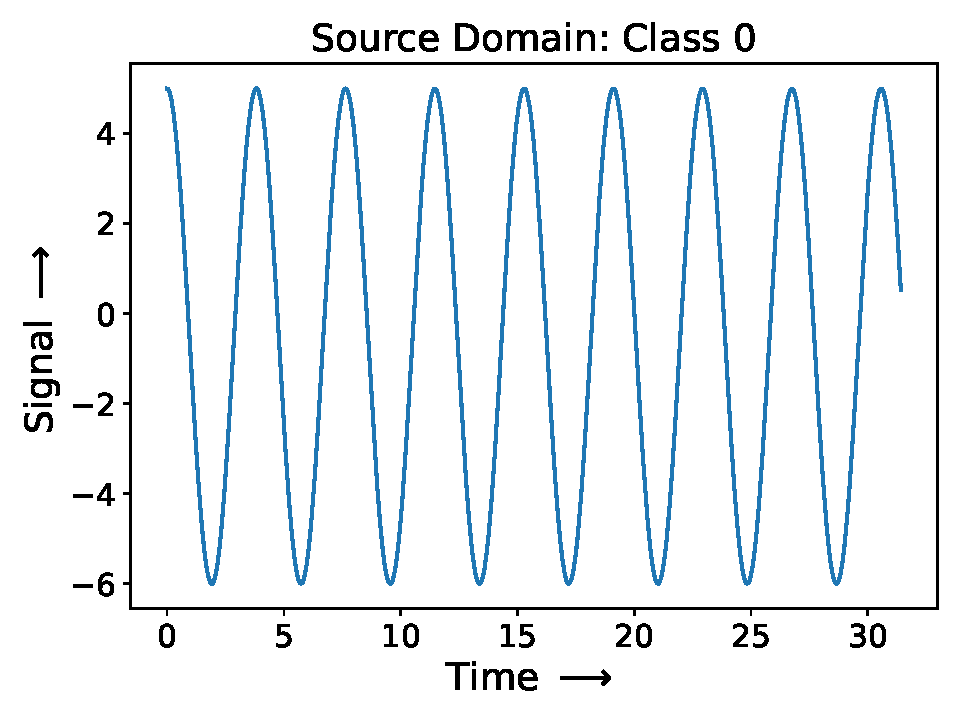
\includegraphics[width=.47\textwidth]{samples_domain_class_dummy_influence_noise/Source_Domain_Class_0_obs_1.pdf}
  \hspace{.3cm}
  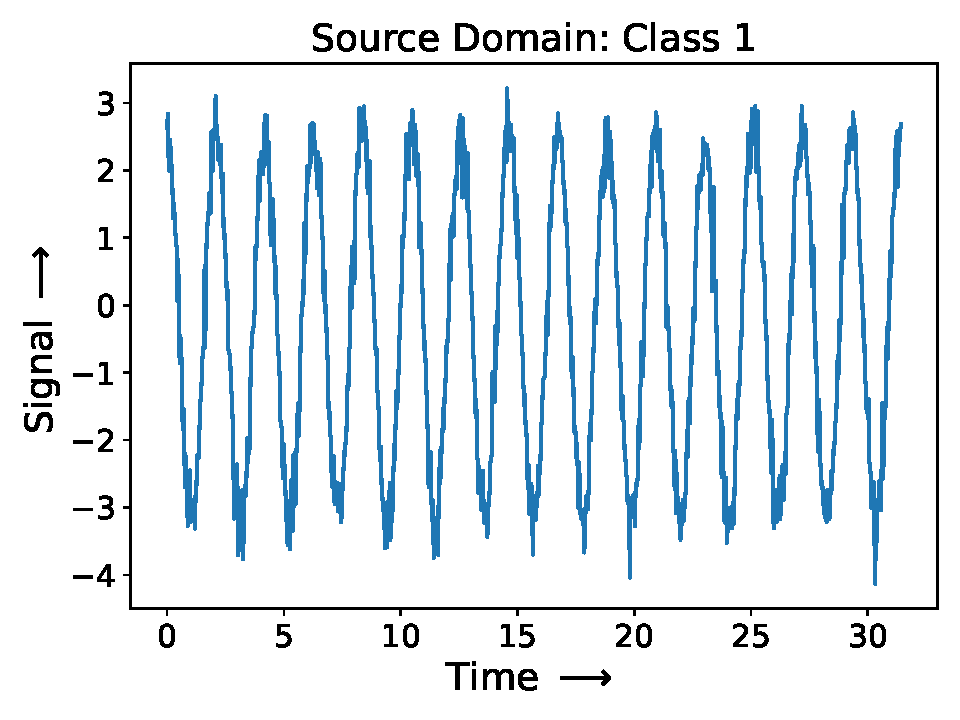
\includegraphics[width=.47\textwidth]{samples_domain_class_dummy_influence_noise/Source_Domain_Class_1_obs_1.pdf}

  \caption{Discrepancy between source samples of equal classes due to applied perturbation and noise during the sampling process}
  \label{fig:samples_domain_class_dummy_influence_noise}
\end{figure}

\section{Ball Screw Feed Drive Dataset} \label{sec:real_world_dataset}
Testing the developed PHM models on a real-world dataset is essential to make statements about the method's utility and applicability for industrial PHM tasks. Milling machines are common in the industry and contain several BSDs, which suffer from degradation. The continuous evaluation of the BSD health condition is therefore essential. A dataset was recorded on an industrial milling machine and the developed PHM models were evaluated by their ability to monitor the health condition of BSDs installed in that machine. In the following, the experimental setup, the mounted sensors, the classification task, the data recording procedure and the resulting PHM task, including a description of the domain shift problem, are presented. 

\subsection{Experimental Setup}
Data from a DMG DMC 55H duoblock milling machine of the manufacturer DMG Mori was recorded. The machine tool’s spindle, machine table, rotary axes, peripherals and the cladding were removed. The TNC control iTNC530 HSCI from Heidenhain GmbH was used. Figure \ref{fig:experimental_setup} shows the experimental setup. The experiments focused on the moving hanger assembly of the machine tool. Generally, the machine tool can move in three spatial directions. The dataset only included data from the machine tool movement along the x-axis. For this reason, the single-threaded screw shaft of the BSD and the two LGSs responsible for that movement were supervised

\begin{figure}[H]
  \centering
  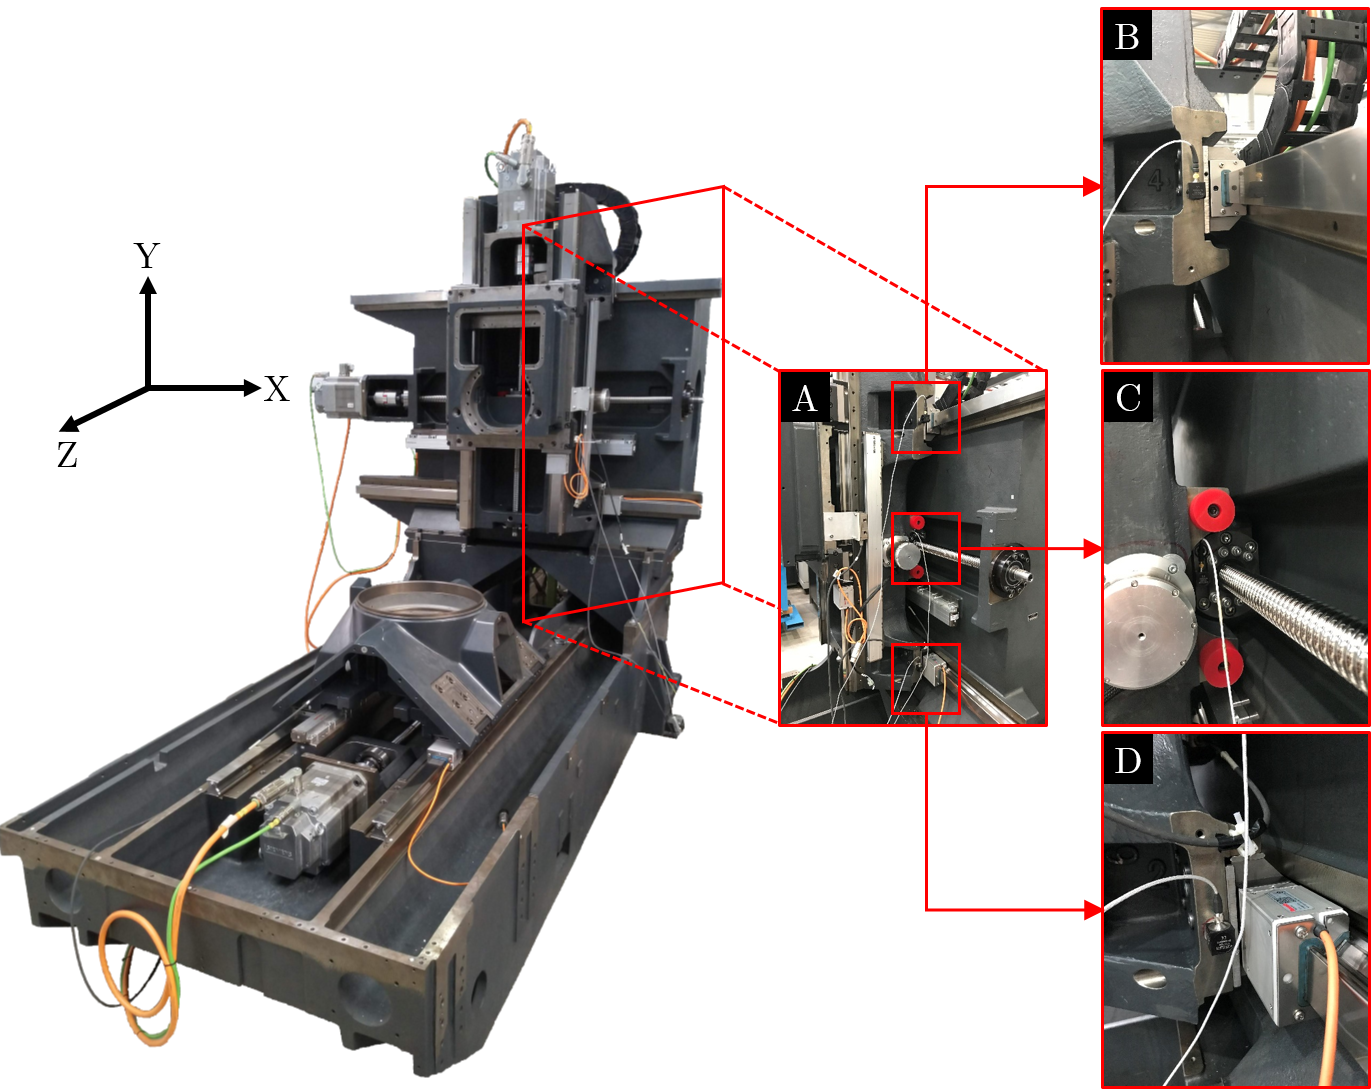
\includegraphics[width=0.9\textwidth]{experimental_setup}
  \caption {Experimental setup: A: side-view of the machine, B: upper LGS, C: threaded screw shaft of BSD, C: lower LGS}
  \label{fig:experimental_setup}
\end{figure}

\subsection{Sensors}
Signals from three different sources were included in the dataset. Three triaxial accelerometers recorded vibration signals and internal control data was accessed via the TNC Scope and TNC Opt. The recordings were triggered by different software programs, which were synchronized by a python script. Minor time delays between the signals could not be eliminated completely. Figure \ref{fig:experimental_setup} shows the placement of the three triaxial Kistler 8762A10 piezo-eletric accelerometers at the upper LGS (sub-figure B), the BSD nut (sub-figure C) and the lower LGS (sub-figure D). The software tool TNC Scope was used to access the internal control data of the machine. TNC Opt is a software tool intended to optimize controllers. During the experiments, it was used to access those control data channels, which differed from those accessible via the TNC Scope.

\subsection{Definition of the Health Condition Classes}
Preload classes (C1, C2, C3) were defined, specifying the preload level in BSDs and LGSs. For the BSDs also pitting damages were observed, which is why a separate pitting class (P) was defined. In total, four health condition classes were defined for the BSDs and three for the LGSs. The degradation of BSDs was specified by an ID containing one letter and either two digits for the preload classes or one digit for the pitting class. The degradation of LGSs was specified by an ID containing one letter and one digit. The letter indicates the damage types: no pitting (C) or pitting (P). The first digit in the BSD preload classes and the single digit in the LGS preload classes specifies the preload level. The second digit in the BSD preload classes and the single digit in the BSD pitting class specifies the observation. The distinct preload classes for the BSDs and LGSs were specified by the preload forces (N) measured in the differently degraded components. Low preload forces result from high preload losses, which indicate strong component degradation. This lowers the precision of the machine and might lead to a complete machine failure. Preload class C3 was labeled as “healthy”, C2 as "slightly degraded" and C1 as "strongly degraded". Two sets of BSDs and one set of LGSs, each containing components of all corresponding health condition classes, were used during the data recording. The observation digit was included in the BSD ID to separate equally degraded BSDs from different sets. In total, ten recordings were made for each BSD and LGS combination. Table \ref{tab:recorded_combinations_of_LGS_and_BSD_health_conditions} shows all 24 combinations of differently degraded and observed BSDs and LGSs. The numbers in table \ref{tab:recorded_combinations_of_LGS_and_BSD_health_conditions} define the specific BSD and LGS combinations and go up to 27. Originally the dataset included a third observation for the BSD preload class 3. In order to prevent a class imbalance, this observation was excluded from the experiments. The preload class definitions differed for the BSD observations. Table \ref {tab:BSDs_states} and table \ref {tab:LGSs_states} show all used BSDs and LGSs, the measured preload forces and the corresponding health condition class IDs. Each experimental setup included two LGSs, each consisting of two counterparts and one BSD. This is the reason why in table \ref {tab:BSDs_states} each ID maps to one and in table \ref {tab:LGSs_states} to four preload forces.

\newpage

\begin{center}
\begin{longtable}{c c c} 
\toprule
 ID & Preload in N \\ [0.5ex] 
\midrule
 P1 & 2 070 \\ 
 P2 & 2 160 \\ 
 C11 & 950 \\ 
 C12 & 845 \\ 
 C21 & 1 450 \\ [1ex] 
 C22 & 1 293 \\ [1ex] 
 C31 & 2 390 \\ [1ex] 
 C32 & 2 328 \\ [1ex] 
\bottomrule
\caption {BSD health condition classes}
\label {tab:BSDs_states}
\end{longtable}
\end{center}

\begin{center}
\begin{longtable}{c c c} 
\toprule
 ID & Component & Preload in N \\ [0.5ex] 
\midrule
 C1 & C1 & 4 060 \\ 
    & C2 & 4 430 \\ 
    & C3 & 4 430 \\
    & F1 & 3 880 \\ 
\midrule
 C2 & B1 & 8 860 \\ 
    & B2 & 9 700 \\ [1ex] 
    & B3 & 9 070 \\ [1ex]
    & E1 & 8 230 \\ [1ex]
\midrule
 C3 & A9 & 13 470 \\ 
    & A10 & 14 530 \\ [1ex] 
    & A11 & 12 840 \\ [1ex]
    & D3 & 12 840 \\ [1ex]
\bottomrule
\caption {LGS health condition classes}
\label {tab:LGSs_states}
\end{longtable}
\end{center}

\begin{comment}
\begin{center}
\begin{longtable}{c c c c c c c c c c} 
\toprule
%\multicolumn{10}{c}{BSD}
&&&&BSD&&&&
\cmidrule(lr){3-11}
  & & C31 & C21 & C11 & P1 & C22 & C12 & C32 & P2  \\ [0.5ex] 
\cmidrule(lr){3-11}
                          & C1 & 1 & 2 & 3 & 4 & 5 & 6 & 7 & 9 \\ 
LGS                       & C2 & 10 & 11 & 12 & 13 & 14 & 15 & 16 & 18  \\ 
                          & C3 & 19 & 20 & 21 & 22 & 23 & 24 & 25 & 27  \\
\bottomrule
\caption {Combinations of LGS and BSD health condition states}
\label {tab:recorded_combinations_of_LGS_and_BSD_health_conditions}
\end{longtable}
\end{center}
\end{comment}






\begin{center}
\begin{longtable}{c c c c c c c c c c} 
\toprule
  &  &    &     &     &     \multicolumn{2}{c}{BSD}     &     &     &    \\ 
  &  & C31 & C21 & C11 & P1  & C22 & C12 & C32 & P2 \\ 
\midrule
     & \multicolumn{1}{c|}{C1} & 1 & 2 & 3 & 4 & 5 & 6 & 7 & 9 \\ 
 LGS & \multicolumn{1}{c|}{C2}& 10 & 11 & 12 & 13 & 14 & 15 & 16 & 18 \\  
     & \multicolumn{1}{c|}{C3} & 19 & 20 & 21 & 22 & 23 & 24 & 25 & 27 \\ 
\bottomrule
\caption {Combinations of LGS and BSD health condition classes}
\label {tab:recorded_combinations_of_LGS_and_BSD_health_conditions}
\end{longtable}
\end{center}


\subsection{Recording of the Dataset}
For reproducibility, the experiments were executed with a fixed test cycle, defined in figure \ref{fig:test_cycle}. The machine data was collected during constant speed, direction change and sweep excitation along the machine tool's X-axis. During the constant speed excitation, the machine tool was moved back and forth along the whole axis ($\Delta x$ = 600mm). During the direction change excitation, the movement of the machine tool was restricted to a small part of the axis ($\Delta x$ = 1mm) and the directions were changed with a high frequency. In the sweep excitation, the motor received a target speed in the form of a sine sweep. Before recording data, the machine was warmed up for 60min with a constant speed to create identical circumstances for all runs. Ten measurement cycles were executed and recorded, each with all three types of excitations. Between each recording the machine was reheated for 2 minutes. 

\begin{figure}[H]
  \centering
  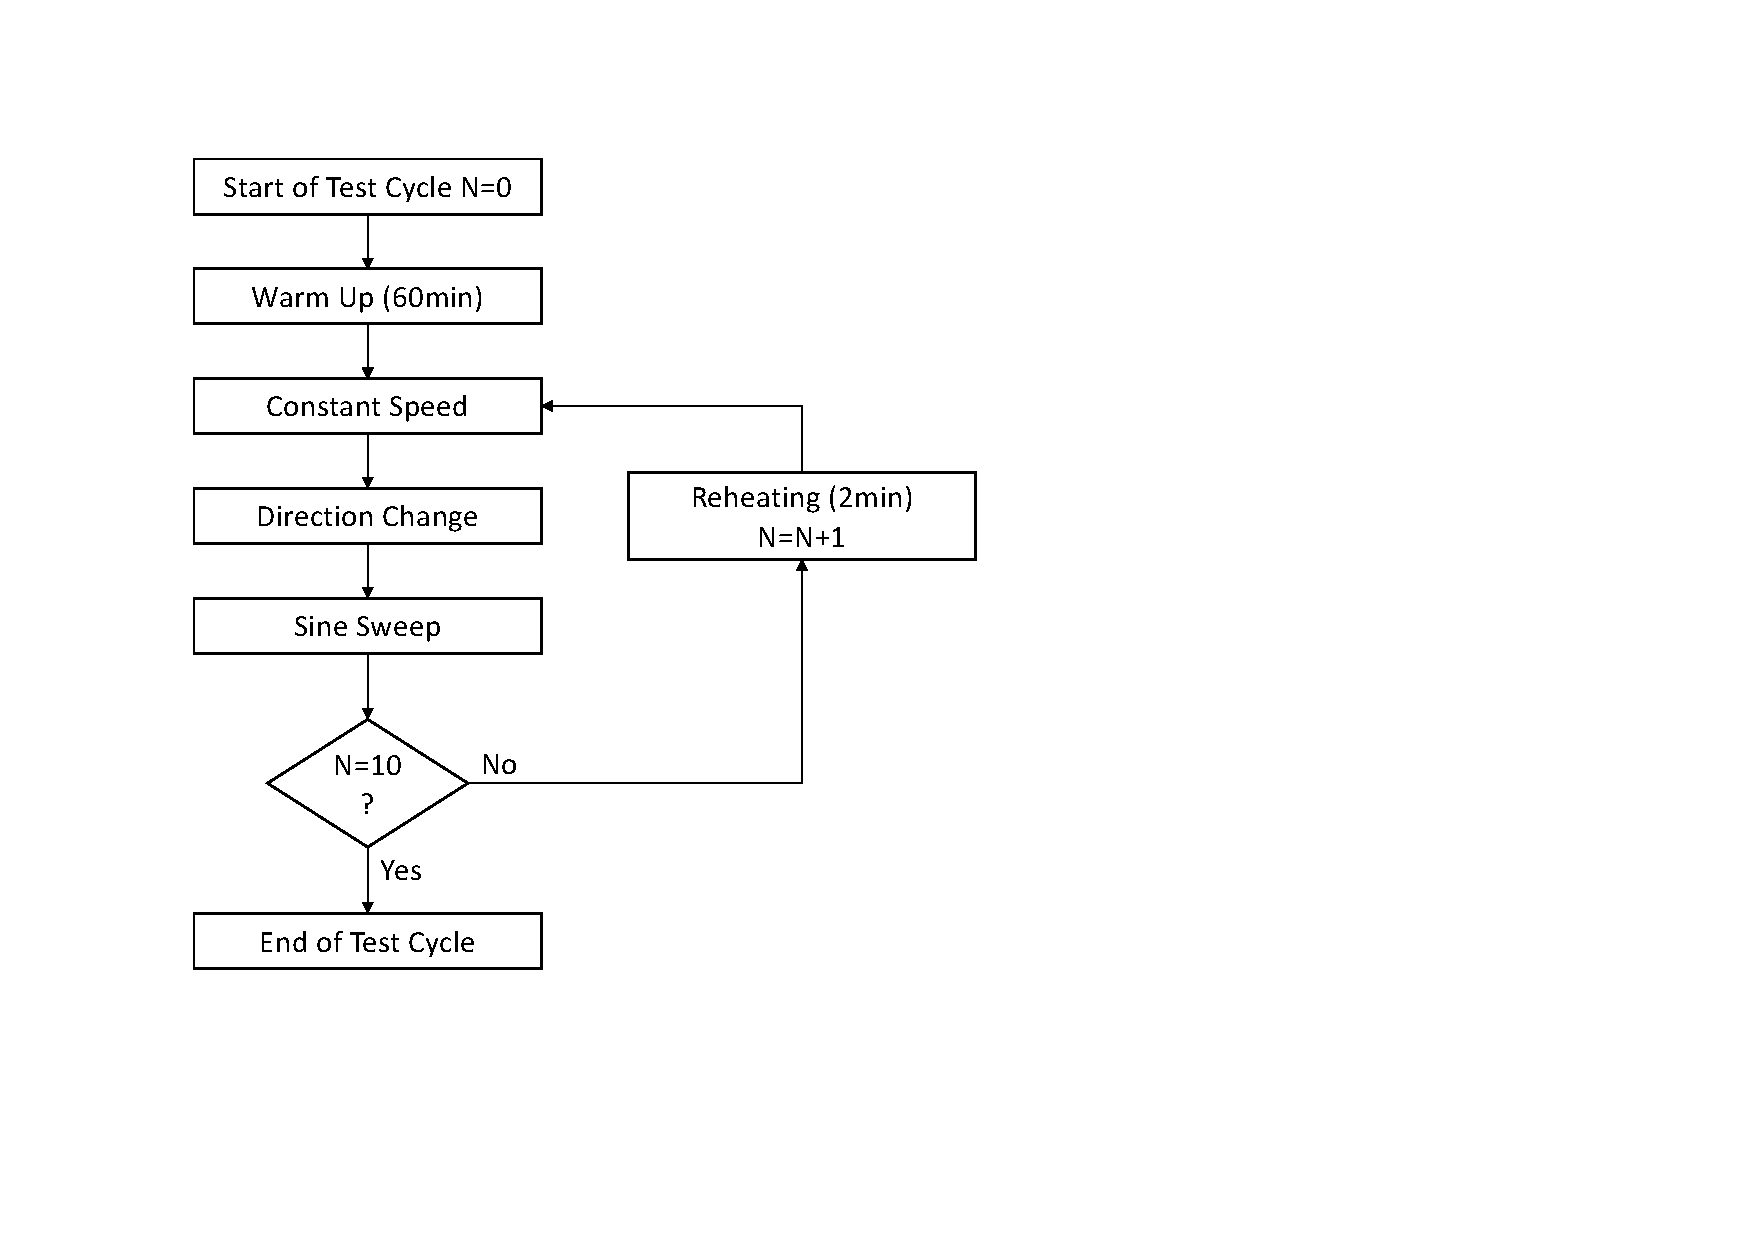
\includegraphics[width=0.6\textwidth]{test_cycle.pdf}
  \caption {Test cycle for data recording}
  \label{fig:test_cycle}
\end{figure}

In total 49 different signals were recorded. A more detailed specification of the signals can be found in the table. \ref{tab:description_of_the_49_recorded_features} in the appendix.

\subsection{Definition of the PHM Task}\label{ch:PHM_Task_Definition}
A binary health condition classification task was created by combining the BSD health condition classes C2 and C3 in a "healthy" and C1 and P1 in a "degraded" class. Therefore, the goal of the proposed model was to predict unacceptable extents of different degradation types (preload loss, pitting damage). A domain shift was generated by combining all samples recorded with BSDs from set 1 (observation digit 1) in the source and set 2 (observation digit 2) in the target domain. Since the measured preload forces differed for the two applied BSD sets (see table \ref{tab:BSDs_states}), a domain shift is guaranteed. Additionally, marginal differences in the production and installation of the BSDs could have increased the domain shift. All combinations of differently degraded LGSs and BSDs were represented in the source and target domain data. 


\section{Methods}\label{sec:methods}
The proposed model architecture and the corresponding training are presented in the following. All models applied to the dummy and real-world datasets had the same architecture. The model training partially deviated from the proposed one during the approaches' pre-evaluation on the dummy dataset. In chapter \ref{sec:results_dummy_dataset}, the training variations are specified in more detail. 

\subsection{Model}
\label{sec:model}
The architecture of the proposed PHM model consists of an one-dimensional CNN and a subsequent classifier. A detailed visualization of the architecture is shown in figure \ref{fig:proposed_model}. The CNN extracts expressive features, which are later used by the classifier to predict the health condition of the BSDs. The CNN consists of three convolutional layers. Throughout the network, the spatial dimension of the feature map is decreased and its depth increased. This helps to extract more global features in shallow and more specific and local features in deeper layers. The exact parameters of the convolutional layers are specified in table \ref{tab:parameter_conv} 
\begin{longtable}{c c c c} 
\toprule
Parameter & Conv 1 & Conv 2 & Conv 3 \\
\midrule
kernel size & 100 & 10 & 5 \\

padding size & 0 & 1 & 1 \\

stride & 1 & 1 & 1 \\
\bottomrule
\caption {Parameters in convolutional layer}
\label {tab:parameter_conv}
\end{longtable}

In order to reduce the spatial dimension of the feature maps, pooling layers are included after the convolutional layers.  The resulting model complexity reduction prevents problems like overfitting and exploding gradients. Batch normalization is applied after the convolutional layers. For each batch, the means and variances of the layers' inputs are fixed, which makes the training faster and more stable. After iteratively applying these three types of layers, the output of the CNN is flattened and normalized to an one-dimensional vector. This vector is fed to the subsequent classifier. The latent feature space dimensions of the classifier are reduced constantly. The probability of the BSD health condition classes is predicted at the end.


\begin{figure}[H]
  \centering
  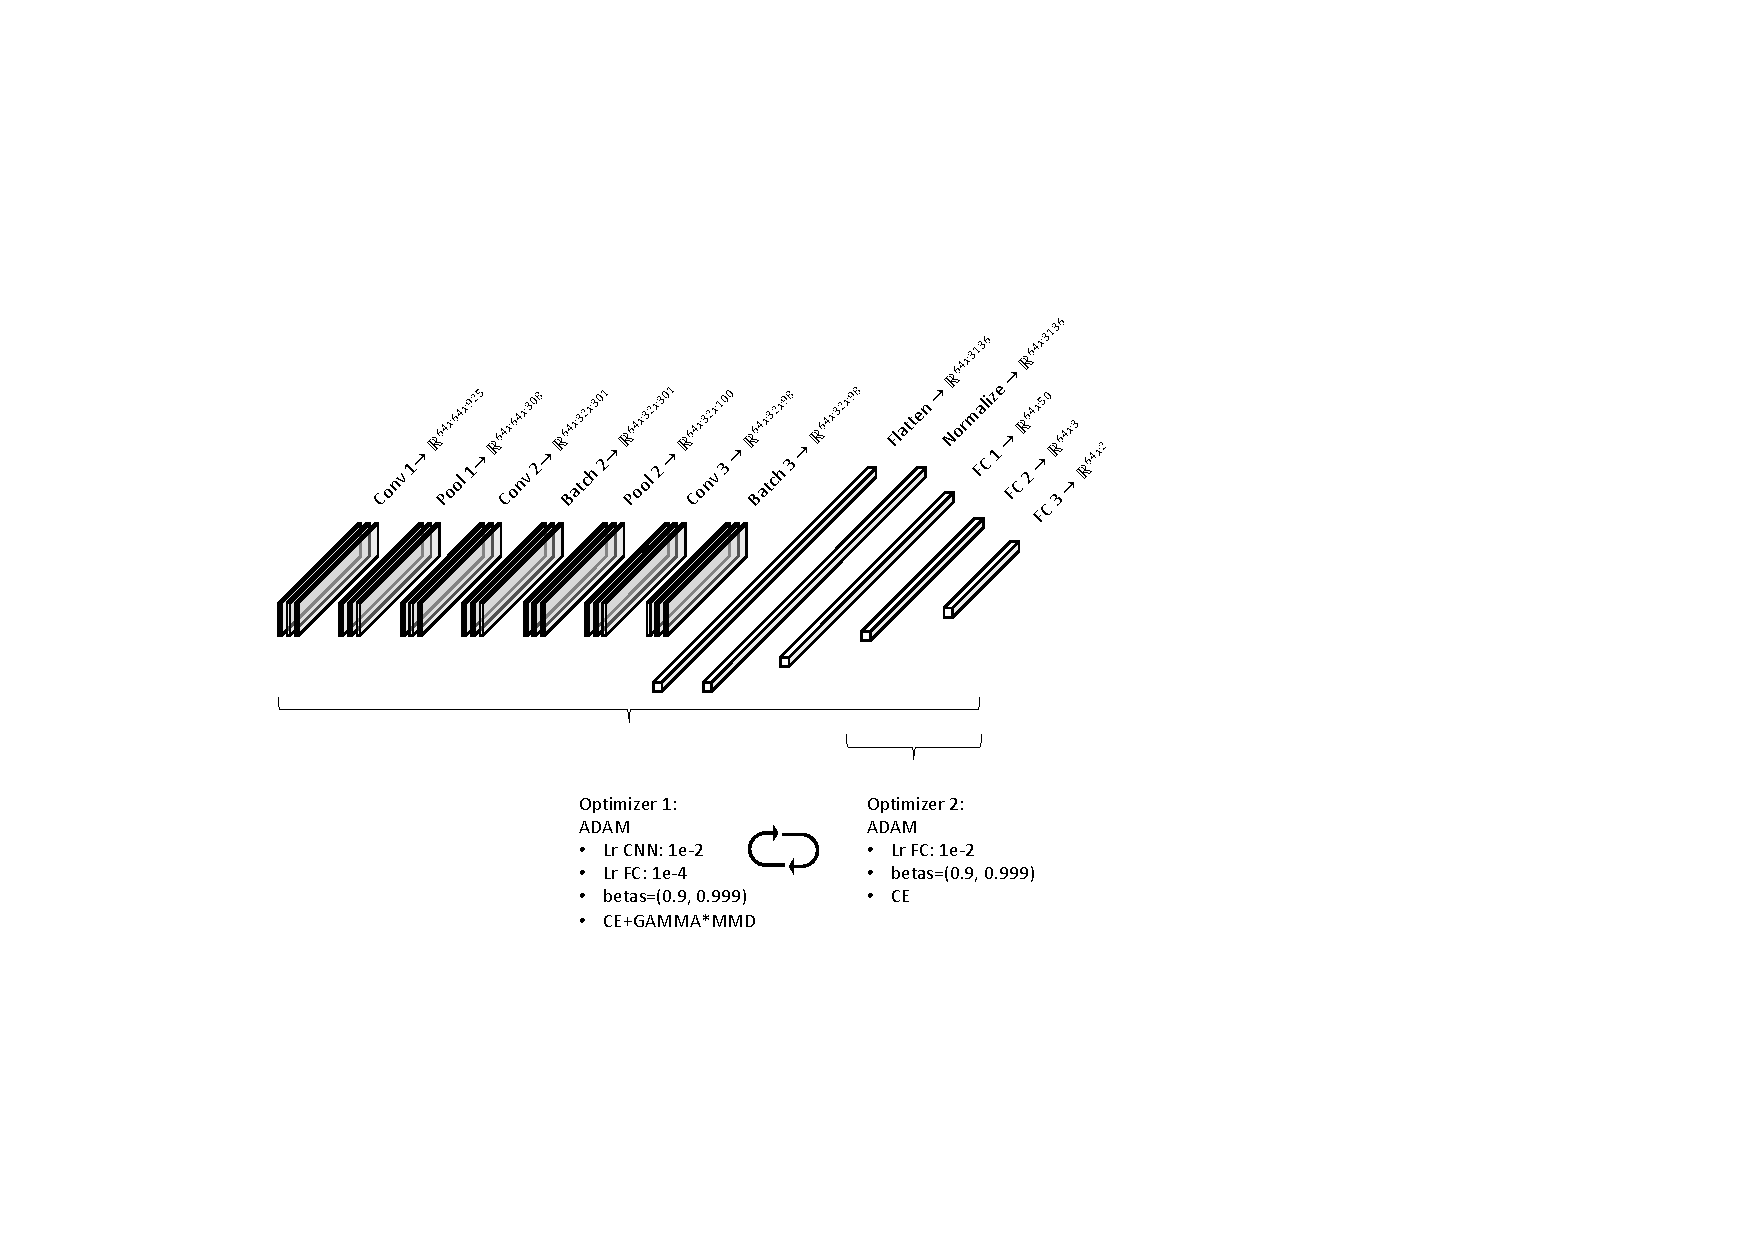
\includegraphics[width=1\textwidth]{proposed_model.pdf}
  \caption {Model architecture} \label{fig:proposed_model}
\end{figure}


\subsection{Model Training} \label{sec:Proposed_training}

In the first step, the data used for the training is pre-processed. In this process, the dataloader separates the data into shorter sequences of length 1024. These windows, which can include several of the recorded 49 signals, are fed to the model as single samples. The sequenced signals are cleaned from Nan values and synchronized afterward. Separate source and target domain dataloaders split the corresponding datasets into four different parts: MMD-Training (40\%), Source CE-Training (20\%), Validation (20\%) and Testing (20\%). Other pre-processing steps, like wavelet transforms, can easily be added to the dataloader. The model training and testing is visualized in figure \ref{fig:Training_Process_MMD}. The repetitive model training is separated into two phases. In the first phase, a weighted average of source CE-loss and MMD-loss is used to optimize the whole network: 
\begin{equation}
    \mbox{Total Loss} = \mbox{Source CE-Loss} + \mbox{GAMMA} \cdot \mbox{MMD-Loss}, 
\end{equation}
where GAMMA is a hyperparameter balancing the influence of the source CE-loss and MMD-loss. Different learning rates in the CNN and classifier allow the training intensity to be adjusted separately for the different modules. In this phase, an ADAM optimizer is applied with a learning rate of 1e-2 in the layers Conv1 - FC1 and a learning rate of 1e-4 in the layers FC2 - FC3. In the second phase, only the source CE-loss is applied to optimize the layers FC2 - FC3. Again an ADAM optimizer with a learning rate of 1e-2 is used. In both optimization steps, the beta values are 0.9 and 0.999. Two-thirds of the training data is used in the first and one-third in the second training phase. The application of the two different optimizers is visualized in figure \ref{fig:proposed_model}.

The MMD-loss estimates the domain discrepancy in the latent feature maps of the neural network. The MMD-loss facilitates the extraction of domain-invariant features. The domain discrepancy is measured as the squared distance between the distribution kernel embeddings in the reproducing kernel Hilbert space (RKHS). The kernel choice is of great importance for the performance of the MMD-loss. By combining several RBF kernels with bandwidth parameters 1, 2, 4, 8, 16, the model training profits from their individual strength. The source and target samples are randomly coupled up and processed by the MMD-loss. The classes of these samples are not considered in the MMD-loss. Therefore, the MMD-loss minimizes the domain discrepancy between source and target domain samples of different and equal classes. The MMD-loss is applied in several layers of the CNN and classifier. The source CE-loss optimizes the model to increase the classification accuracy on the source domain data. Figure \ref{fig:MMD_Loss_and_CE_loss} symbolically shows how the MMD and the source CE-loss are applied in different model layers. The training is repeated until the maximum number of epochs is reached. After the training is completed, the model can be used to predict the BSD health condition classes of unseen target domain samples. 



\begin{figure}[H]
  \centering
  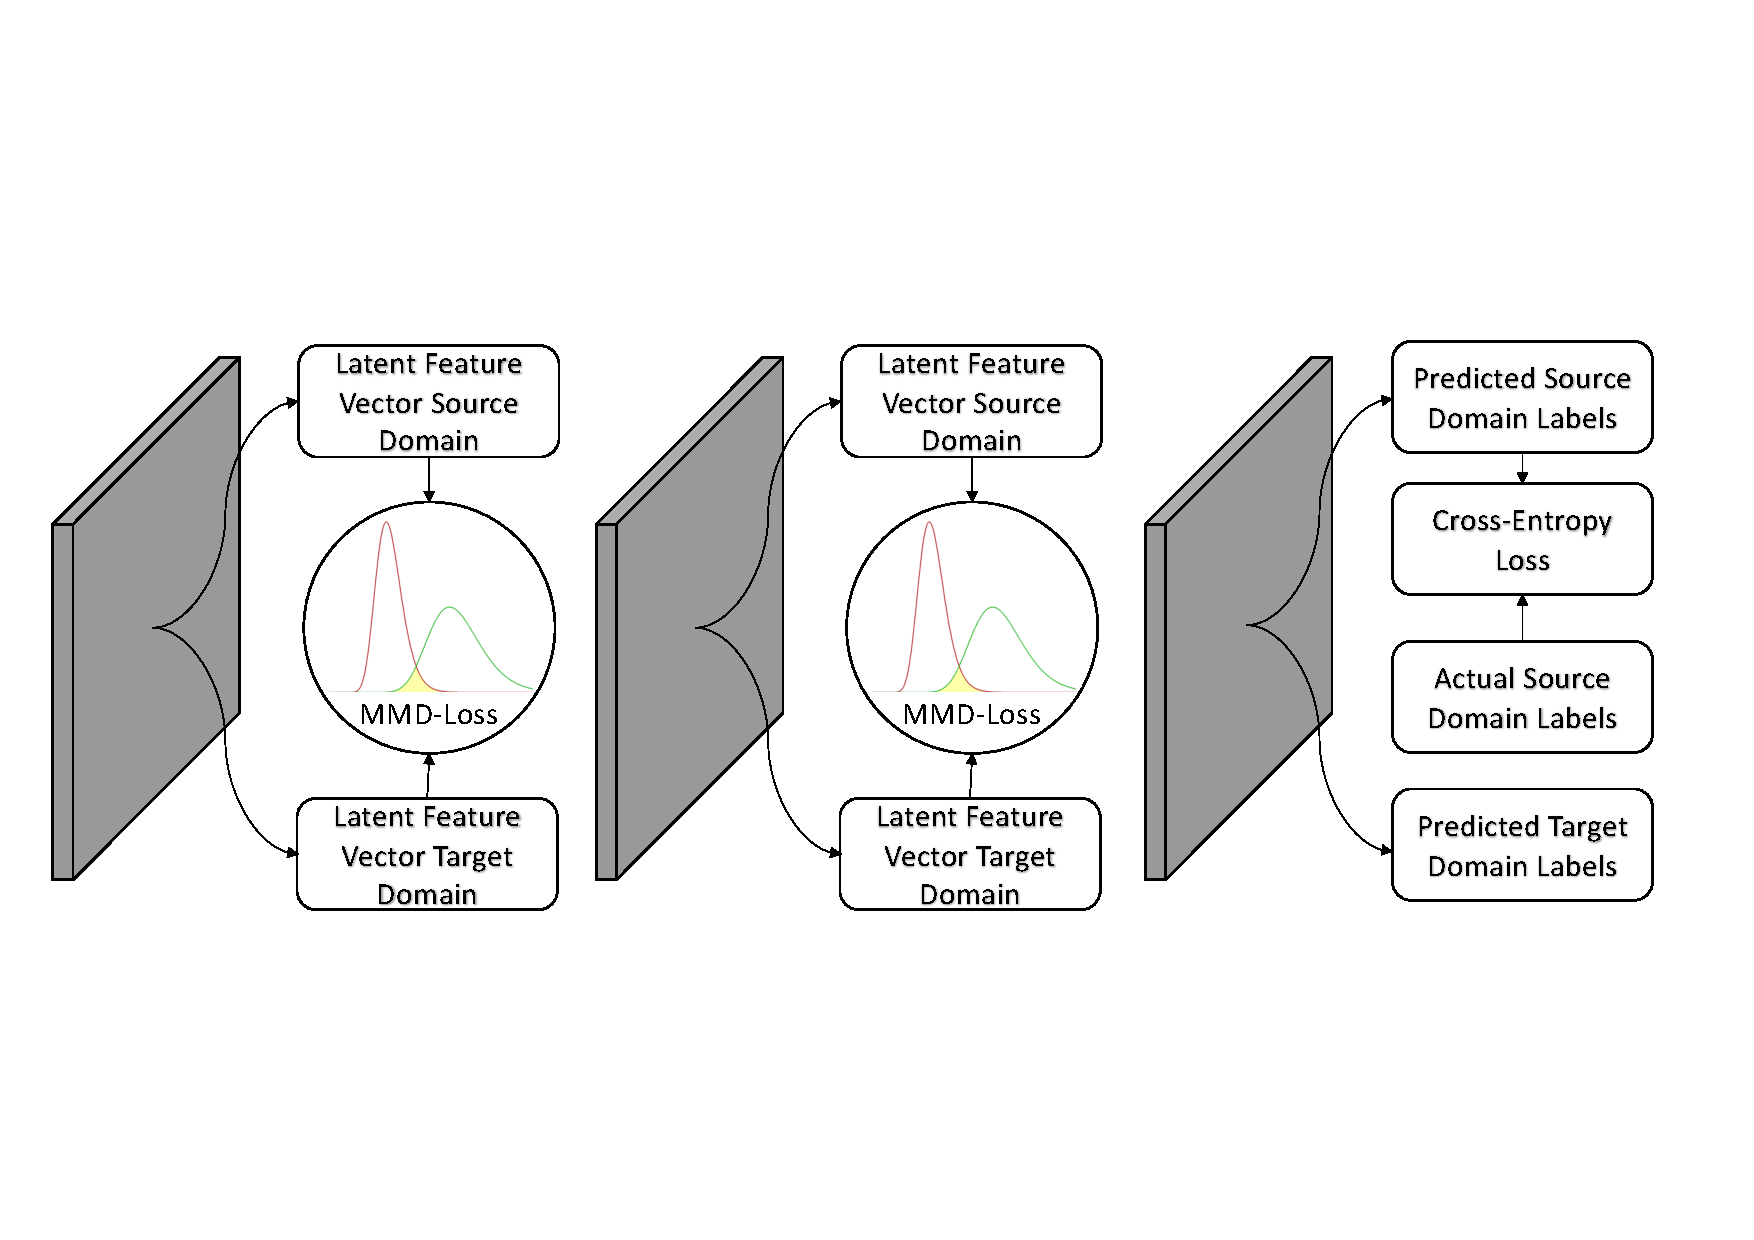
\includegraphics[width=1\textwidth]{MMD_loss_visualization.pdf}
  \caption {Optimization of neural networks with a source CE- and MMD-loss} \label{fig:MMD_Loss_and_CE_loss}
\end{figure}

\begin{figure}[H]
  \centering
  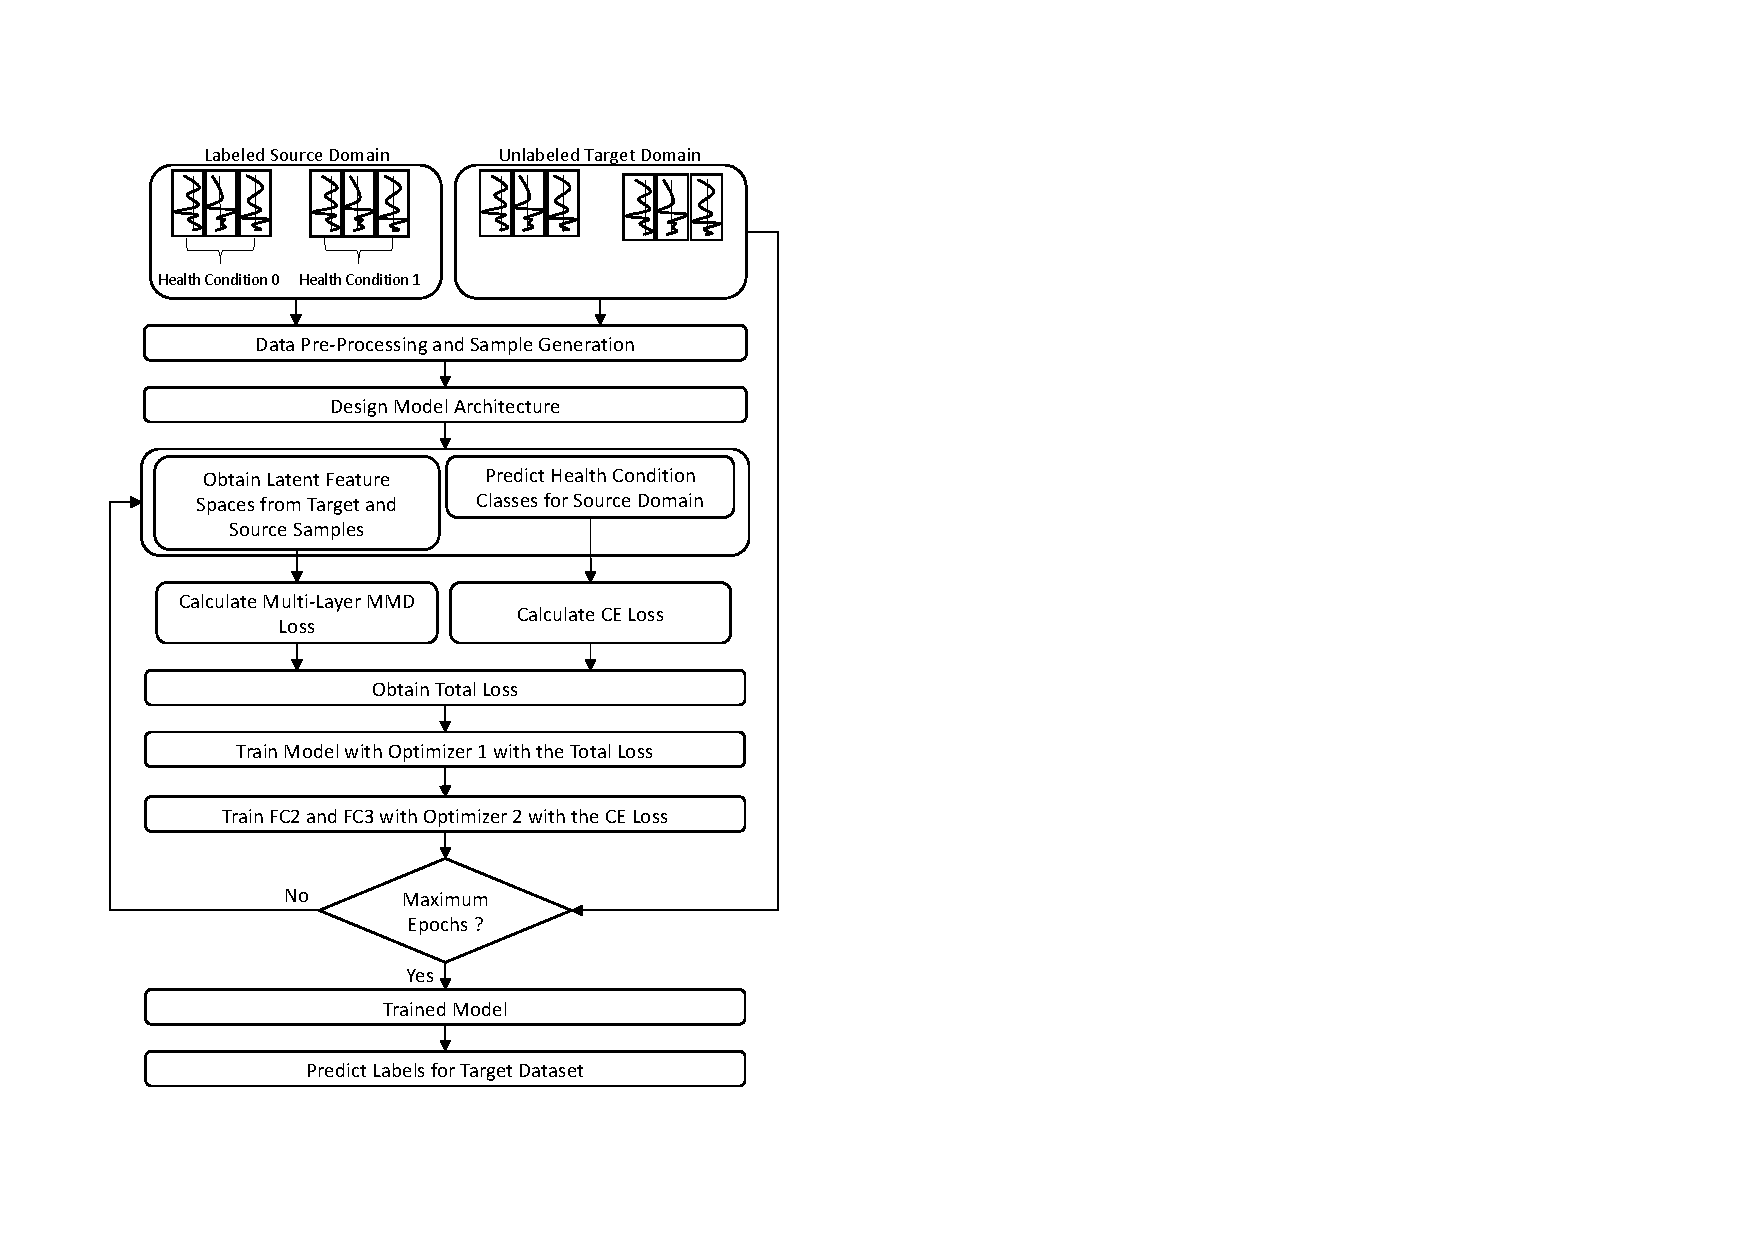
\includegraphics[width=0.8\textwidth]{training_process_mmd.pdf}
  \caption {Model training and testing} \label{fig:Training_Process_MMD}
\end{figure}

